\documentclass[a4paper]{panl}


\usepackage{cite}
\usepackage{wrapfig}
\usepackage{graphicx}
\usepackage{amssymb}
\usepackage{amsfonts}
\usepackage{amsmath}
\usepackage{longtable}
\usepackage{rotating}
\usepackage{lscape}
\usepackage{epsfig}
\usepackage{multirow}



\originalTeX
%\russianTeX
\begin{document}
% Journal sections (see http://pkp.jinr.ru/index.php/PEPAN_LETTERS/about/editorialPolicies#focusAndScope)
\issuearea{Physics of Elementary Particles and Atomic Nuclei. Theory}
% or in Russian
%\issuearea{ФИЗИКА ЭЛЕМЕНТАРНЫХ ЧАСТИЦ И АТОМНОГО ЯДРА. ТЕОРИЯ}

\title{Chemical composition analysis for X-ray transport container scans.  \\ Анализ химического состава при сканировании транспортных контейнеров гамма-излучением}
\maketitle
\authors{A. Zelenaya$^{~a}$, M. Zelenyi$^{~a,b,}$\footnote{E-mail: mihail.zelenyy@phystech.edu}, A.A.Turinge$^{~a}$,  V.G. Nedorezov$^{~a,}$\footnote{E-mail: vladimir@cpc.inr.ac.ru}}
\from{$^{a}$\,Institute of Nuclear Research of RAS}
\vspace{-3mm}
\from{$^{b}$\,Moscow Institute of Physical and Technology  (SU)}

\begin{abstract}
% Russian translation of the abstract
It is important for national security to control the movement of dangerous or strategically cargo such as explosives, radioactive materials, rare and precious metals. This control can be provided by scanning transport containers by gamma rays.
In this report the existing technique for scanning (dual energy method) is considered and the alternative method based on measuring the energy distribution of gamma rays is proposed. For estimation perspectives of the proposing method, the  corresponding simulation was conducted by using the GEANT4 toolkit. The example of the algorithm of reconstruction the chemical composition of the scanned object is also considered. In addition the experiment for estimation energy resolution of the detector based on a scintillation crystal BGO and SiPM was carried out.\\
\vspace{0.2cm}

Для обеспечения национальной безопасности важен контроль перемещения опасных или стратегически важных грузов, таких как взрывчатые вещества, радиоактивные материалы, редкие и драгоценные металлы. Проводить такой контроль можно сканирую содержимое   транспортных контейнеров гамма излучением. В данной работе рассмотрена существующая методика дуальных энергий и предложен альтернативный способ, основанный на измерении энергетического распределения гамма-квантов. Для оценки было проведено моделирование с помощью транспортного кода GEANT4.  Также выполнен эксперимент по измерению энергетического разрешения детектора на основе сцинтиллирующего кристалла BGO и кремневого фотоумножителя. 
\end{abstract}
\vspace*{6pt}

\noindent
PACS: 02.70.$-$c; 23.20.Nx; 32.90.$+$a

\newpage
\label{sec:intro}
\section*{Introduction}
Geant4~\cite{ALLISON2016186, spirin}
\section*{Dual energy method}
Consider how the flux of gamma rays decreases. Прозрачность (transmittance) описывается следующей формулой:
\begin{equation}
\label{eq:trans}
T(E_0, t, Z) = \frac{\int \limits_0^{E_0} S(E_0, E) \exp(-\mu(E,Z)\times t)~dE)}{\int \limits_0^{E_0} S(E_0, E)~dE},
\end{equation}
where $T$ -  transmittance, $S(E_0, E)$ - response function, $\mu(E,Z)$ - attenuation, $t$ -  optical thickness of material, $E_0$ -  up-limit energy of bremsstrahlung, $E$ - energy of gamma ray, $Z$ - charge of nuclei.
We assume that bremsstrahlung is used as a source of gamma rays, with a spectrum, for example, as in figure~\ref{fig01}b and with the maximum energy depending on the energy of the electron beam. Our transmittance also depends on the mean material attenuation coefficient. Figure~\ref{fig01}a shows the dependence of the attenuation coefficient on energy for different materials. We can distinguish three areas: the initial one in which the photoelectric effect dominates and only materials with a large nuclear charge stand out; the average in which Compton scattering dominates and materials are not distinguishable, and the area where the main influence is produced by the production of electron-positron pairs, and the materials are quite well distinguishable. The last area can be used for the dual energy method.
\begin{figure}[t]
\begin{center}
    % Сделать подписи к отдельным картинкам
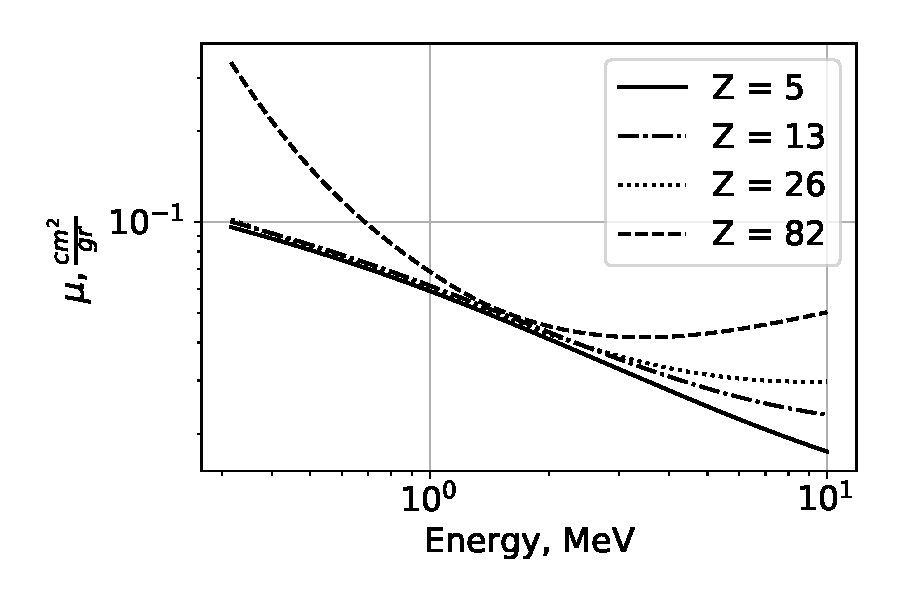
\includegraphics[width=60mm]{figures/Attenuation.pdf} 
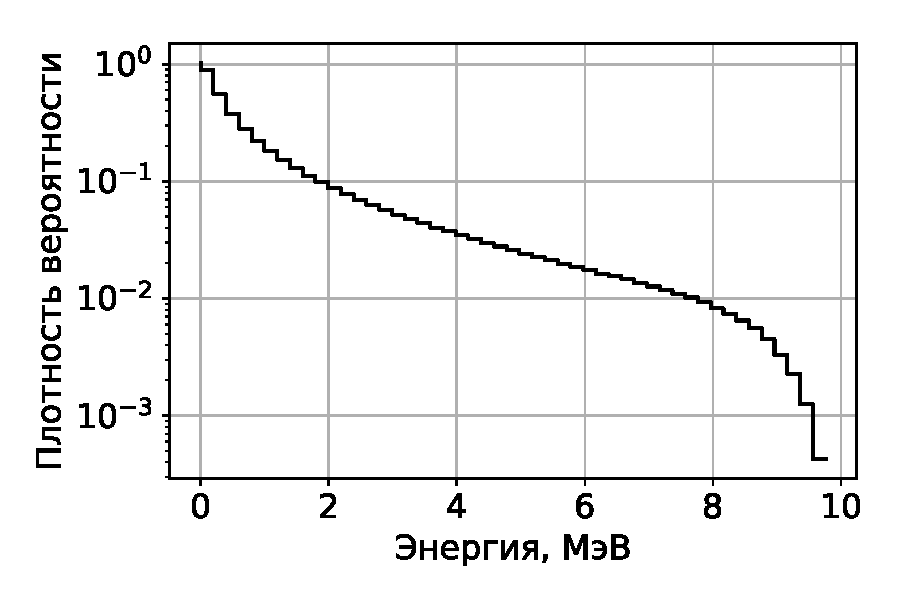
\includegraphics[width=60mm]{figures/Bremsstrahlung.pdf}  
\vspace{-3mm}
\caption{a)Attenuation curve b) Bremsstrahlung spectrum by $10 MeV$ electron}
\end{center}
\labelf{fig01}
\vspace{-5mm}
\end{figure}
The dual energy method is based on using two electron beams with different energies. Since the equation from the previous slide does not determine the nuclear charge, if the optical thickness of the material is not known, to solve this problem, we consider the transmittance for the two limit energies of gamma rays $E^{(1)}_0$ and $E^{(2)}_0$, and then minimizing this functional:
\begin{equation}
F(z) = \frac{|t(E^{(1)}_0,z) - t(E^{(2)}_0,z)|}{t(E^{(1)}_0,z)} \to min
\end{equation}
we exclude unknown optical thickness from consideration and determine the average charge of the material. This method allows to determine which of these four groups the scanned object belongs to. This technique allows to determine scan object as a one from four possible groups: $Z_{eff} \sim 5$, $Z_{eff} \sim 13$, $Z_{eff} \sim 26$, $Z_{eff} \sim 82$.\\
This method has several disadvantages:
    \begin{itemize}
        \item It is too difficult to irradiate the target with beams with different energy.
        \item Low efficiency for target which contains elements with strongly different charges.
    \end{itemize}
Therefore, we offer an alternative method:
    \begin{itemize}
        \item Use only one electron beam with energy $E = 10 MeV$.
        \item Measure not only the space distribution, but also the energy of gamma rays.
    \end{itemize}

\section*{Simulation}
\begin{figure}[t]
    \begin{center}
        % Сделать подписи к отдельным картинкам
        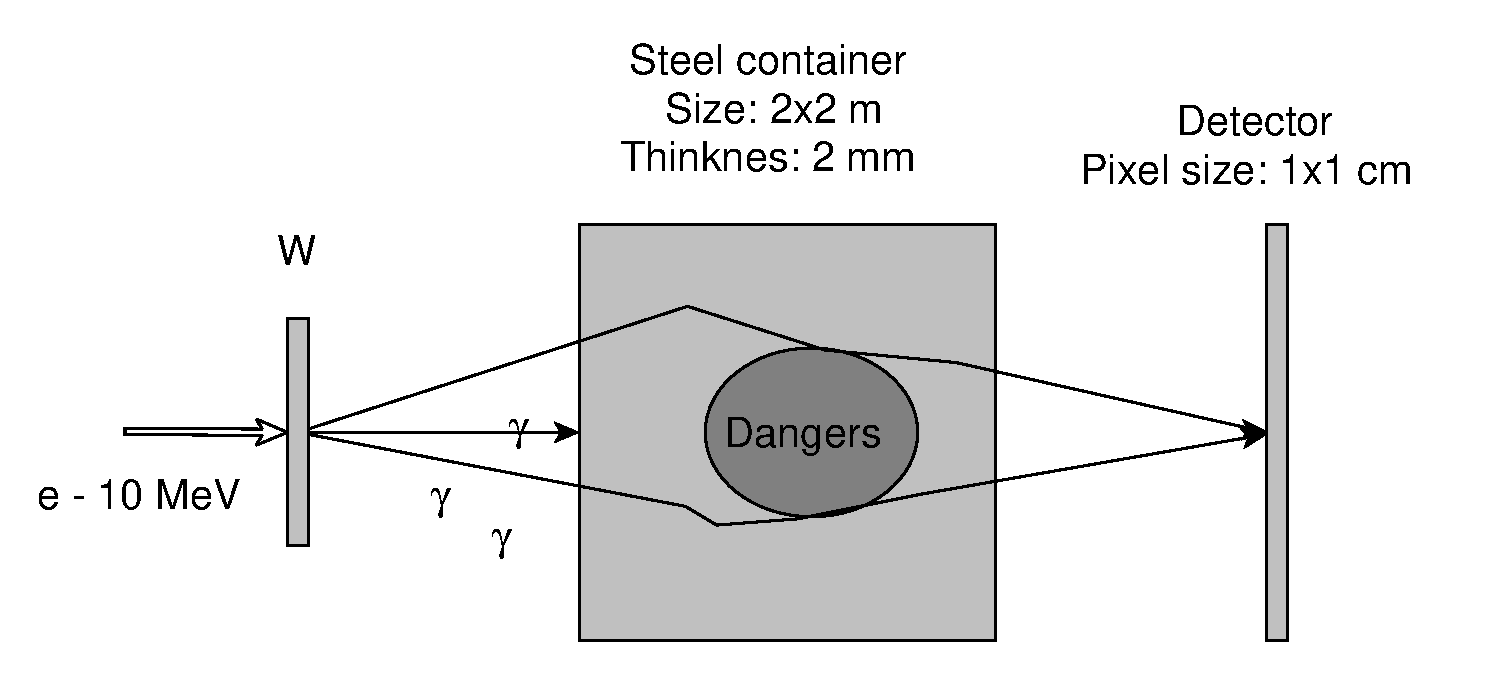
\includegraphics[width=120mm]{figures/yed_schema_1.pdf}
        \vspace{-3mm}
        \caption{a) }
    \end{center}
    \labelf{pic:schema1}
    \vspace{-5mm}
\end{figure}
For evaluation, we conducted several simulations using the scheme (fig.~\ref{pic:schema1}):
An electron beam with the energy of 10 MeV collides with a wolfram converter, producing a bremsstrahlung that irradiates a steel two-meter container, inside which the object under study is located and is detected by a detector. Расcтояние между вольфрамовым конвертером и контейнером два метра, между контернером и детектором 10 см. Приведем некоторые примеры моделирования.
\begin{figure}[t]
    \begin{center}
        % Сделать подписи к отдельным картинкам
        % Переделать картинку от Туринге
        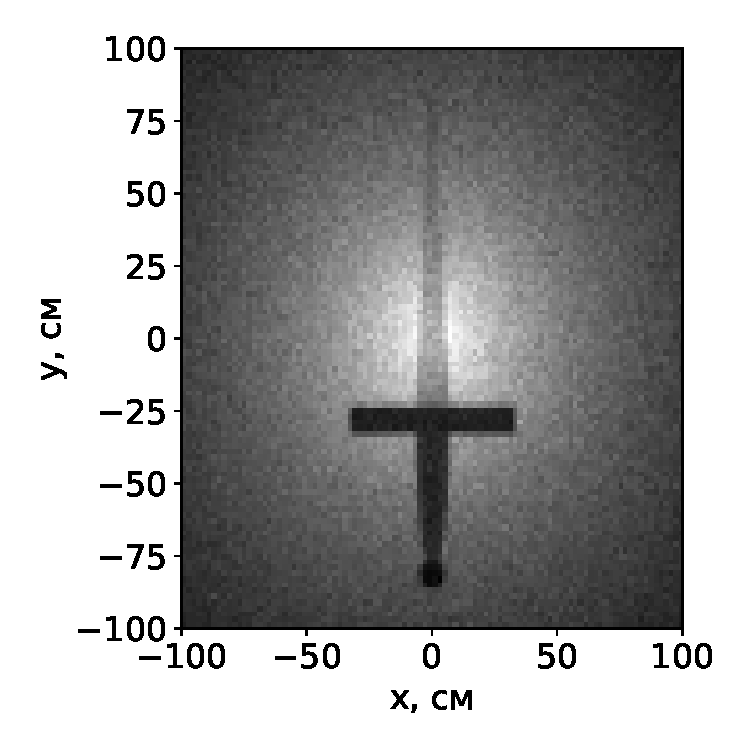
\includegraphics[width=60mm]{figures/Sword.pdf} 
        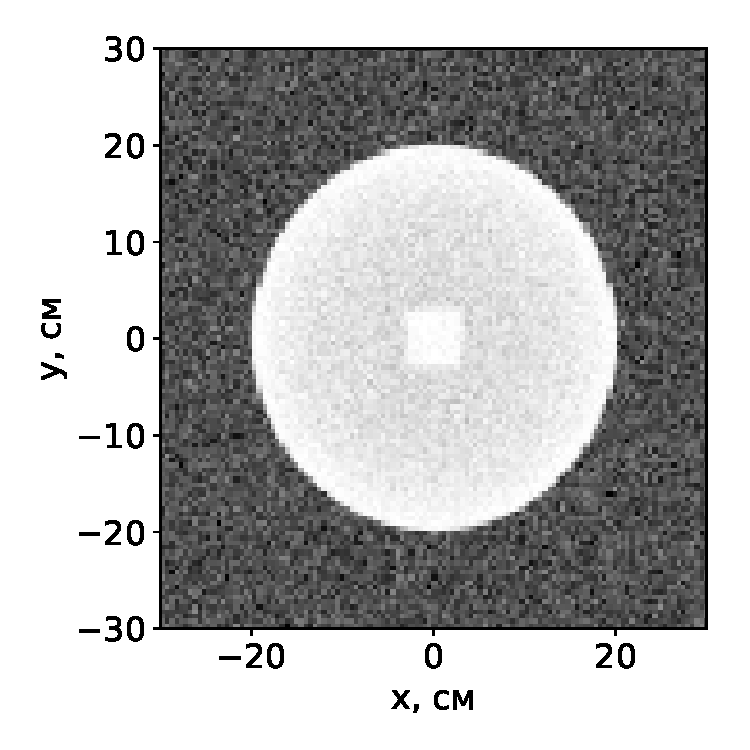
\includegraphics[width=60mm]{figures/UranCube1.pdf}  
        \vspace{-3mm}
        \caption{a) b)}
    \end{center}
    \labelf{pic:sword}
    \vspace{-5mm}
\end{figure}
\begin{figure}[t]
    \begin{center}
        % Сделать подписи к отдельным картинкам
        % Переделать картинку от Туринге
        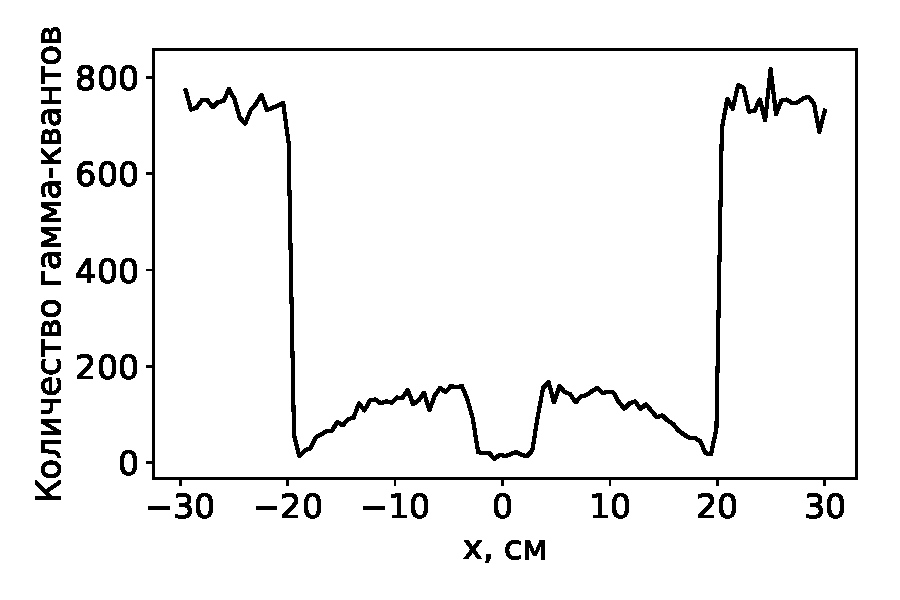
\includegraphics[width=60mm]{figures/UranCube2.pdf} 
        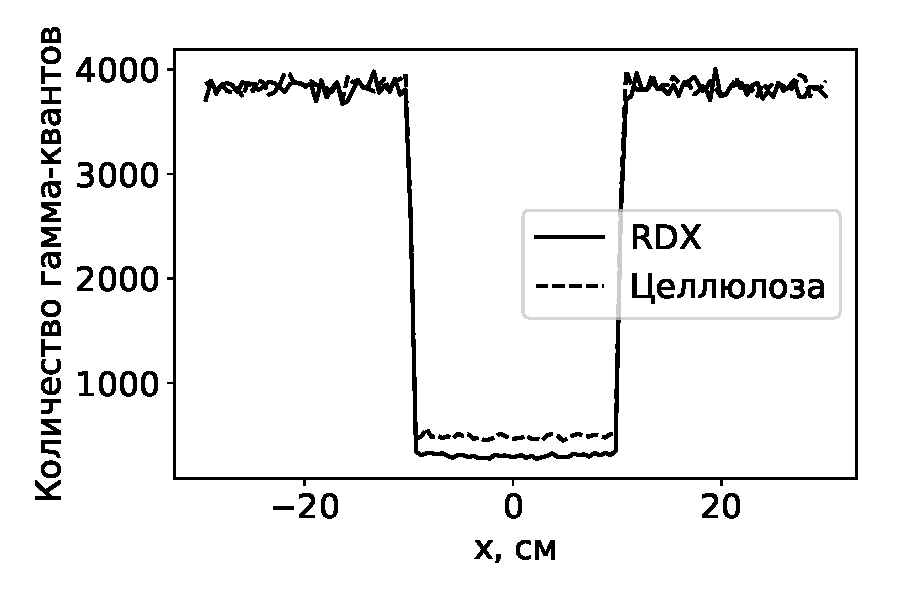
\includegraphics[width=60mm]{figures/Hex.pdf}  
        \vspace{-3mm}
        \caption{a) b)}
    \end{center}
    \labelf{pic:hex}
    \vspace{-5mm}
\end{figure}
\begin{figure}[t]
    \begin{center}
        % Сделать подписи к отдельным картинкам
        % Переделать картинку от Туринге
        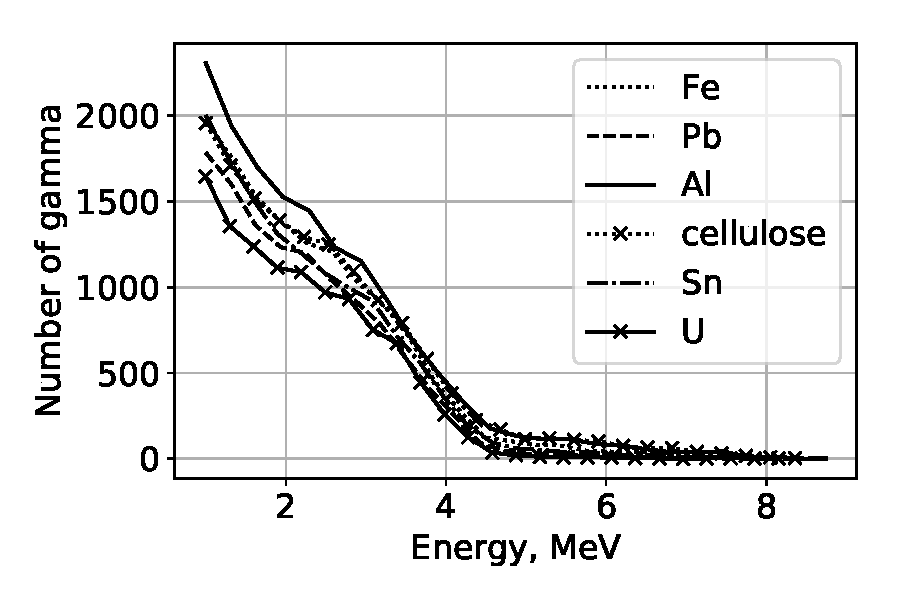
\includegraphics[width=60mm]{figures/diffmat0.pdf} 
        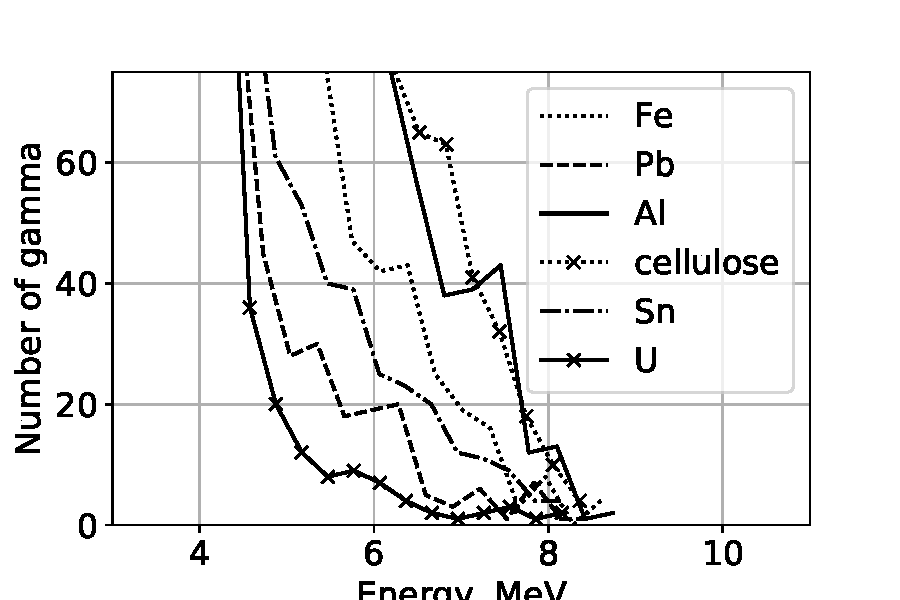
\includegraphics[width=60mm]{figures/diffmat.pdf}  
        \vspace{-3mm}
        \caption{a) b)}
    \end{center}
    \labelf{fig01}
    \vspace{-5mm}
\end{figure}
\begin{figure}[t]
    \begin{center}
        % Сделать подписи к отдельным картинкам
        % Переделать картинку от Туринге
        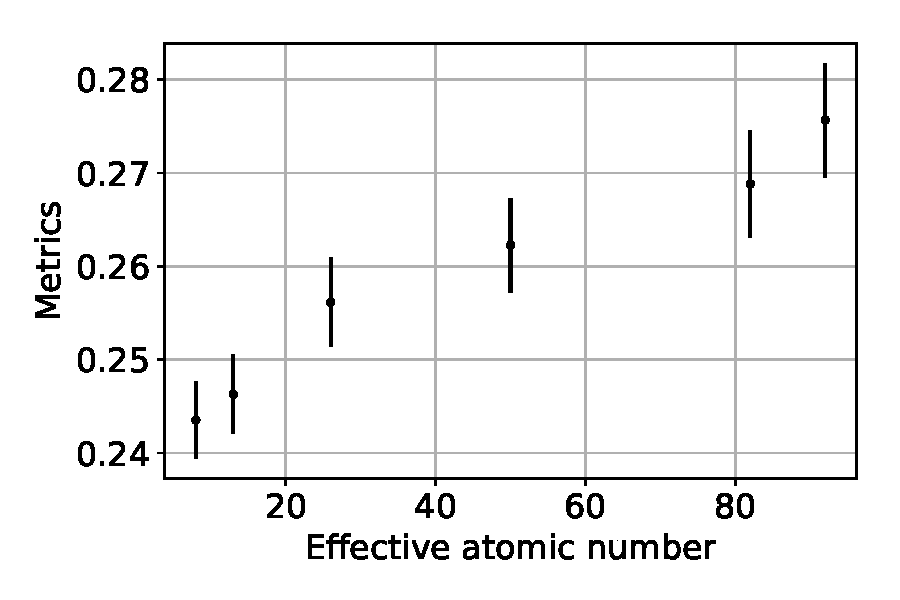
\includegraphics[width=60mm]{figures/diffmat1.pdf} 
        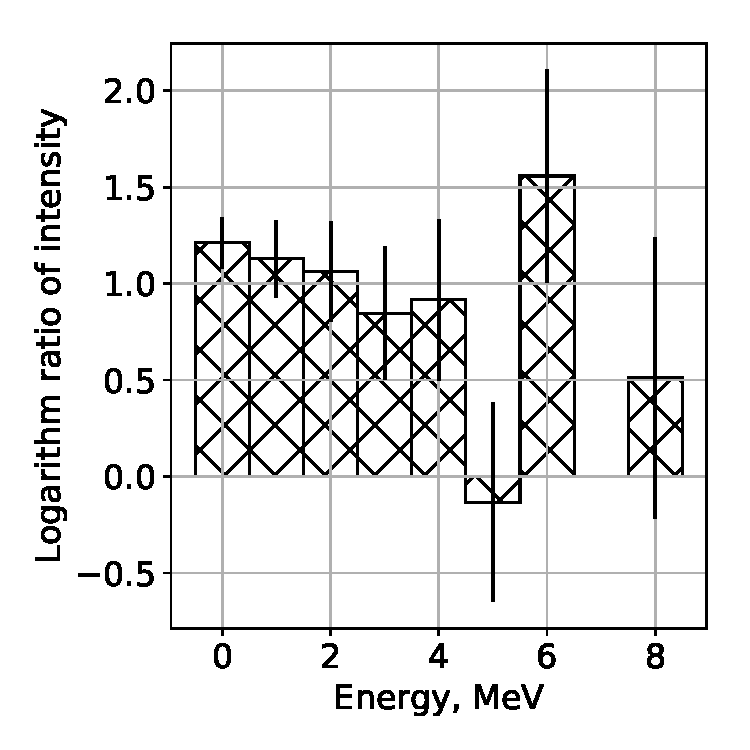
\includegraphics[width=60mm]{figures/Difference.pdf}  
        \vspace{-3mm}
        \caption{a) b)}
    \end{center}
    \labelf{pic:diff}
    \vspace{-5mm}
\end{figure}
На рисунке ~\ref{pic:sword})a пример опасного предмета из стали неравномерной толщины близкой к толщине стенок контейнера. На рисунках~\ref{pic:sword}b и ~\ref{pic:hex}a  показан результат  моделирования кубика урана с ребром 6 сантиметров (масса около 4 кг), помещённого в свинцовую сферу толщиной 1 см, как показало моделирования такой куб можно обнаружить при толщине оболочки вплоть до 5 сантиметров. Рисунок ~\ref{pic:hex}b демонстрирует различие между двумя органическими материалами: безопасным - целлюлозы, и опасным  - RDX. Различие значимо, а значит есть возможность создать алгоритмы поиска органических взрывчатых веществ. На рисуноке ~\ref{pic:diff}b  показывается результат сравнения двух энергетических спектров (в  качестве метрики выбран логарифм отношения интенсивностей) от алюминиевого и уранового шариков диаметром 1 см. Как мы видим даже на таких малых масштабах и небольших (по сравнение с реальным пучком) интенсивностях возможна регистрация различий в энергетических спектрах.


\section*{Thickness reconstruction}
\begin{wrapfigure}[9]{r}{0.6\linewidth} 
    % Сделать подписи к отдельным картинкам
    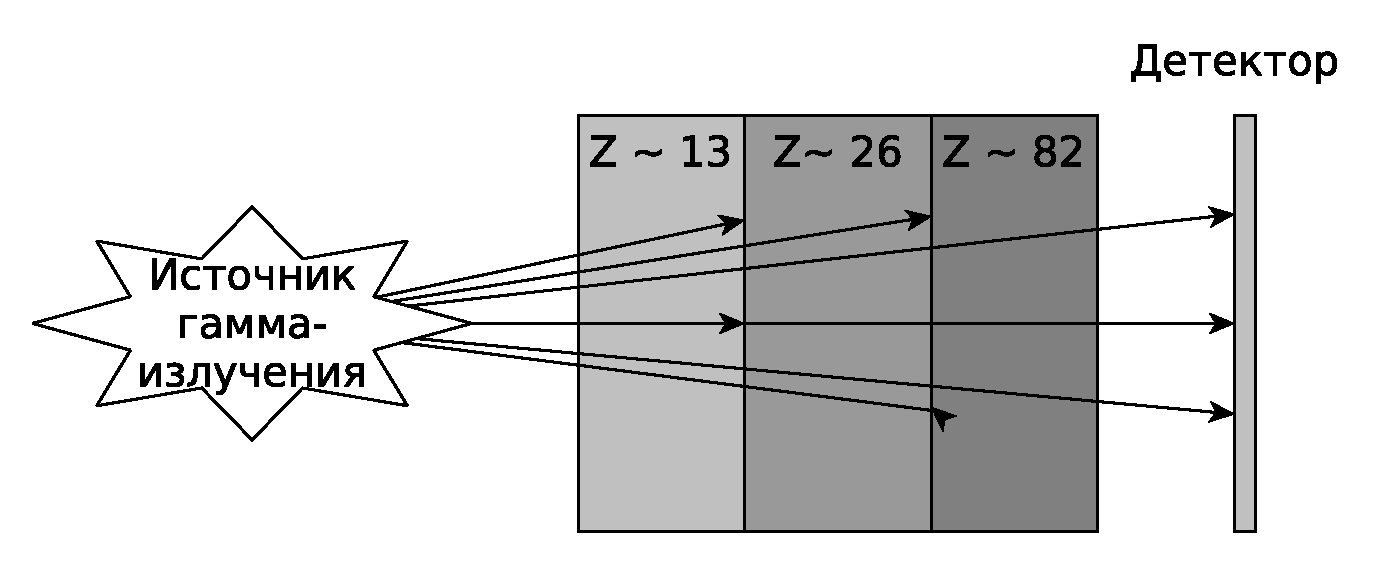
\includegraphics[width=\linewidth]{figures/yed_schema_2.pdf}
    \vspace{-3mm}
    \caption{ Thickness reconstruction}
    \labelf{schema2}
    \vspace{-5mm}
\end{wrapfigure}
Мы будем рассматривать одномерный случай, когда гамма-кванты проходят скозь стопку из нескольких материалов с фиксированной полной толщиной и нам нужно восстановить толщины отдельных материалов (см. схему ~\ref{scema2}). Мы будем использовать простую физическую модель в которой ослабление задается  следующей формулой: 
\begin{equation}
\label{eq:gamma}
\frac{N(E)}{N_0(E)} = \exp(-\sum_i \Sigma^{mean}_i(E)x_i),
\end{equation}
where $x_i$ --- thickness of the $i$-layer, $\Sigma^{mean}_i$ --- mean cross-section for group of materials with близкими зарядами ядра, $N,~N_0$ --- the number of gamma.При этом мы не будем учитывать множественное рассеяние и наличие аннигиляционной линии. Мы считаем что полная толщина известна и для восстановления толщин отдельных слоев мы будем использовать метод наименьших квадратов, то есть минимизировать такую сумму:
\begin{equation}
\sum_E(\ln \frac{N(E)}{N_0(E)} + \sum_i \Sigma^{mean}_i(E)x_i))^2 \to min
\end{equation}
Далее приведен пример работы алгоритма. We consider the object which has 3 layers of aluminium, iron and lead.The figure~\ref{rec:ex}a shows a contribution of every reconstructed material in summary attenuation. The table~\ref{tab:rec} contains the results of reconstruction.As we can see from the table, its result is quite accurate. To clarify the capabilities of the algorithm, we conducted several numerical experiments.We also used aluminum, iron and lead, but now we have taken many sets of thicknesses, with a total thickness between 30 and 180 centimeters. The figure~\ref{rec:ex}b shows the variation of recovery errors for these sets. As we can see, the thickness of heavy elements is determined best of all - with an accuracy about 5\%, and worst of all for materials from the iron group, the error there reaches 30\%. However, this is too simple model. What good will it do? We used only the energy distribution, if we also add a space distribution, then we can try to reconstruct the three-dimensional structure of the cargo in the container (the 3D gamma tomography). Therefore, our simple model shows that we have the prospect of creating a truly powerful system for analyzing the contents of containers.
\begin{figure}[t]
    \begin{center}
        % Сделать подписи к отдельным картинкам
        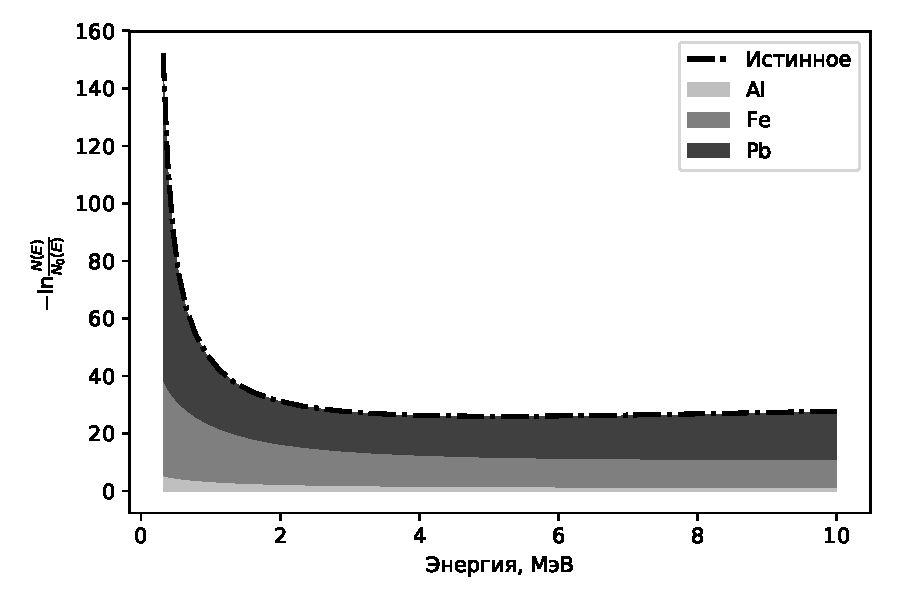
\includegraphics[width=60mm]{figures/reconstruction.pdf} 
        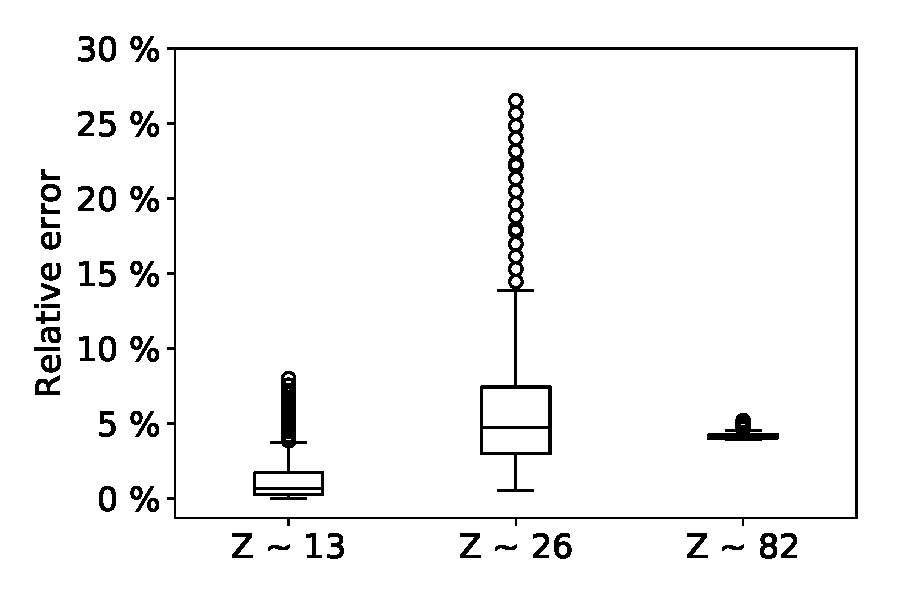
\includegraphics[width=60mm]{figures/relError.pdf}  
        \vspace{-3mm}
        \caption{a) b)Distribution of reconstruction errors for various numerical experiments}
    \end{center}
    \labelf{rec:ex}
    \vspace{-5mm}
\end{figure}

\begin{table}
\begin{center}
        \begin{tabular}[c]{|c|c|c|}
        \hline 
        Material & Real, cm & Reconstructed, cm \\ 
        \hline 
        Al & 20 & 19.6 \\ 
        \hline 
        Fe & 40 & 41.6 \\ 
        \hline 
        Pb & 30 & 28.7 \\ 
        \hline 
    \end{tabular}
\end{center}
\caption{Example of thickness reconstruction}
    \label{tab:rec}
\end{table}


\section*{Experiment}
\begin{wrapfigure}[14]{r}{0.5\linewidth} 
    % Сделать подписи к отдельным картинкам
    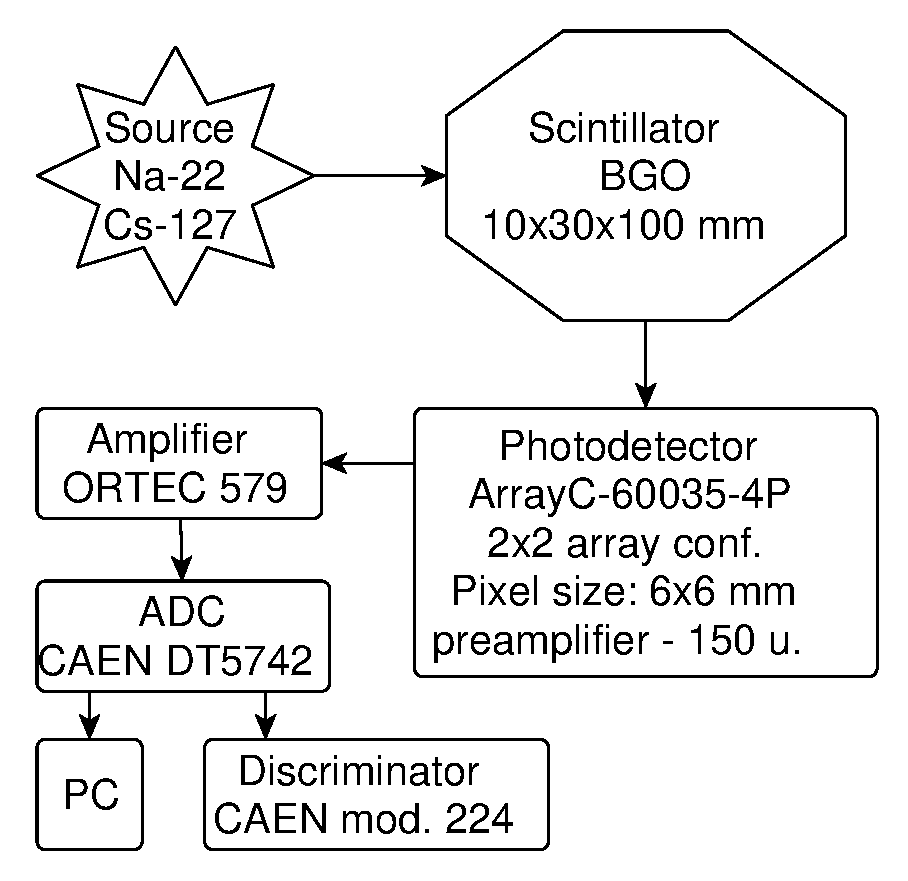
\includegraphics[width=\linewidth]{figures/yed.pdf}  
    \vspace{-3mm}
    \caption{Schema of experiment}
    \labelf{pic:experiment}
    \vspace{-5mm}
\end{wrapfigure}
Кроме моделирования, доктором Губером и доктором Ивашкины, проведены измерения энергического разрешения детектора  для регистрации гамма излучения. Схема эксперимента приведена на рисунке~\ref{pic:experiment}. В работе использовались сцинтиллятор BGO размером 10х30х100мм и фотодетектор ArrayC-60035-4P. Проводились измерения спектров от источников $\beta$– излучения (Na-22 и Cs-137). Энергии излучения 0.511 МэВ и 1.275 МэВ для Na и 0.662 МэВ для Cs. В качестве фотодетектора использовалась матрица из четырех фотодиодов ArrayC-60035-4P с размером фотодиода 6х6мм, снабженная индивидуальным предусилителем с коэффициентом усиления 150. В процессе работы измерялся суммарный сигнал с двух фотодиодов матрицы. Сигнал c матрицы подавался на усилитель (ORTEC 579) и затем поступал на входной канал АЦП (CAEN DT5742) и на дискриминатор (CAEN mod.224), логический сигнал которого служил триггером в системе. В отсутствие источника шкала АЦП была прокалибрована в абсолютных единицах – числе фотоэлектронов. Результат измерения энергитического разрешения приведен в таблице ~\ref{tab:ex}

The experiment was conducted by Dr. Guber and Dr. Ivashkin.
The sum of signals from 2 photodiode\\
Noise threshold: 100 KeV\\
\begin{table}
    \begin{center} 
        \begin{tabular}[c]{|c|c|c|}
            
            \hline 
            Source & Energy, MeV & Sigma/Mean \\
            \hline 
            $^{22}Na$&0.511 & 14.7\%  \\ 
            \hline 
            $^{137}Cs$&0.662 & 19\%\\ 
            \hline 
            $^{22}Na$& 1.275 & 13\% \\
            \hline 
        \end{tabular} 
    \end{center}
\caption{Energy resolution of detector}
\label{tab:ex}
\end{table}


\section*{Conclusion}
% Выводы сделать более твердыми и акцентирванными
Results:   
    \begin{enumerate}
        \item The measurement of the gamma ray spectrum allows to identify cargo belonging to the group of materials with certain $Z_{eff}$.
        \item Also it allows to define the thickness of layers from different elements with the accuracy about 25\%.
        \item The energy resolution of the detector based on a BGO scintillator was studied.  For the photodetector with full array of pixels the energy resolution is expected about 10\%.
    \end{enumerate}
Plans and perspectives
    With financial support can be developed:
    \begin{enumerate}
        \item The program which checks cargo of a transport container  for compliance cargo manifest
        \item The algorithm for the 3D gamma-tomography.
    \end{enumerate}

This work is supported by the Ministry of Education and Science of the Russian Federation under the contract No. 3.3008.2017/PP.


%============================= Fig. 1 ================================
%\begin{figure}[t]
%\begin{center}
%\includegraphics[width=127mm]{fig_1.eps} 
%%\includegraphics[width=127mm]{fig_1.eps} 
%\vspace{-3mm}
%\caption{Figure caption}
%\end{center}
%\labelf{fig01}
%\vspace{-5mm}
%\end{figure}
%============================= Fig. 1 ================================


%\nocite{*}
\bibliographystyle{pepan}
\bibliography{references.bib}

\end{document}
